\begin{section}[Refining UR with NLP]{Refining User Representation with NLP}
\begin{frame}{Refining User Understanding in Recommendation via NLP}
\begin{columns}
  \begin{column}{.35\textwidth}
  \onslide<1->{
  \begin{block}{\centering  Intuition}
    \centering  Reviews can help improve recommendation performances \& make predictions understandable.
    \end{block}
    }
     \onslide<2->{
    \begin{block}{\centering Approach}
    \begin{center}
        Traditional rating regression \\
    +\\
    attentive sentiment analysis
    \end{center}
    \end{block}
    }
  \end{column}
    \begin{column}{.65\textwidth}
     \onslide<2->{
        \begin{figure}
            \centering
            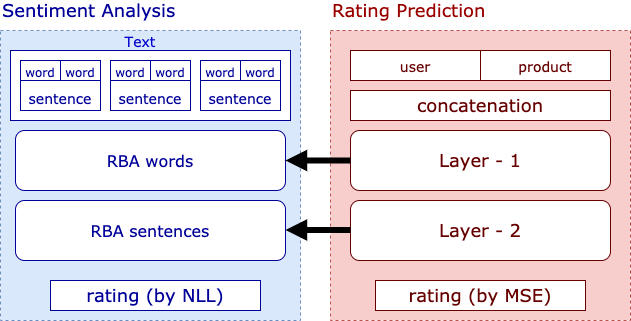
\includegraphics[width=\textwidth]{img/coriaModel.png}
            \caption{General view of the Hierarchical Recurrent Attentive Network (HRAN).}
             \label{fig:coriaOverview}
        \end{figure}
        }
  \end{column}
\end{columns}
    
\end{frame}

\begin{frame}{Model - RBA}
    \begin{figure}
        \centering
        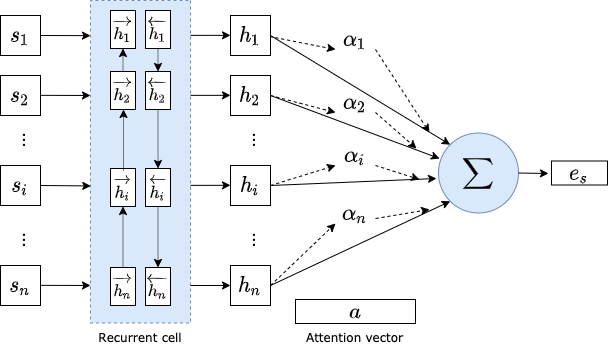
\includegraphics[height=.7\textheight]{img/RBA.png}
        \caption{Recurrent Bi-directional Attention Module, based on the work of \cite{yang2016hierarchical}.}
        \label{fig:coriaOverview}
    \end{figure}
\end{frame}

\begin{frame}{Model - Details}
    \begin{figure}
        \centering
        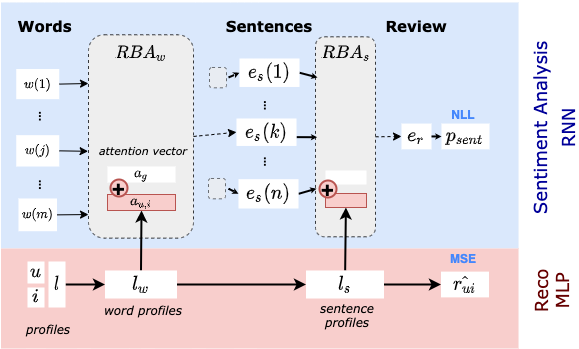
\includegraphics[height=.8\textheight]{img/globalArchOverviewCoria.png}
        \caption{ \centering Detailed view of the model for an input of $n$ sentences of $m$ words.}
        \label{fig:coriaOverview}
    \end{figure}
\end{frame}

\begin{frame}{Results - RMSE}
    \begin{table}[t]
    \centering
    \begin{tabular}{@{}llllll@{}}
    \toprule
    Dataset  (\#reviews)        & Mean $(\mu)$  & w/offset & FM 	& TransNet & HRAN  \\ \midrule
    Instant Video  (37.126)     & 1.25 			&  1.137   &    1.024   & 1.526 	&\textbf{0.937} \\
    Digital Music (64,706)      & 1.19	 		&   0.965  &    0.903 	& 1.522 	& \textbf{0.838}  \\
    Video Games  (231,780)      & 1.45	 		&   1.281  & 	1.267  	& 1.313  	&  \textbf{1.076} \\
    CSJ (278,677)               & 1.215 		&   1.323  &    1.365	& 1.285 	&  \textbf{1.081} \\
    Movie (1,697,533)           & 1.436	 		&   1.148  &    1.118 	& 1.359  	& \textbf{1.058} \\
    \bottomrule
    \end{tabular}
    \titlecaption{\centering RMSE in rating prediction}{} \label{tab:recoRMSE}
\end{table}
\end{frame}
% \begin{frame}{Results, Sentiment Analysis}
%     \begin{table}[t]
    \centering
    \begin{tabular}{@{}lllll@{}}
    \toprule
                        & FastText  &  HAN  & NSUPA  & HRAN         \\ \midrule
    Instant Video       & 62.60        & 64.50 &   65.88   & \textbf{66.60}          \\
    Digital Music       & 63.58        &   68.03   &   \textbf{70.08}   & 68.80          \\
    Video Games         & 62.51       &   67.67  &   68.60   & \textbf{69.11}            \\
    CSJ	                & 67.83        &    71.96  &   \textbf{71.99}   & 71.49          \\
    Movies              & 64.56       &   68.95   	&   71.20   & \textbf{71.62 }           \\\bottomrule
    \end{tabular}
    \titlecaption{\centering Accuracy metric on the sentiment analysis task}{}\label{tab:sentacc} 
    \end{table}
% \end{frame}

\begin{frame}{Attention Visualization}
    \begin{figure}[t]
    \begin{minipage}[c]{.48\linewidth}
        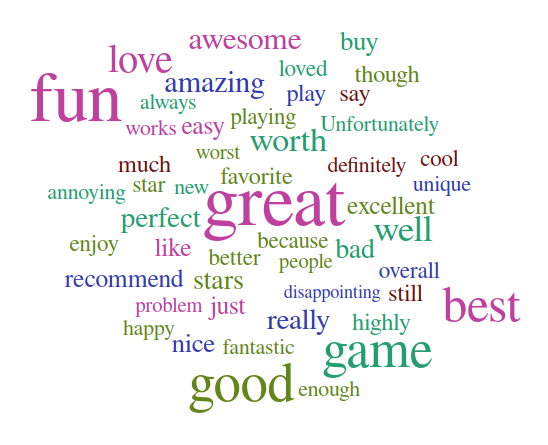
\includegraphics[width=\linewidth]{img/adj.png}
    \end{minipage} \hfill
    \begin{minipage}[c]{.48\linewidth}
        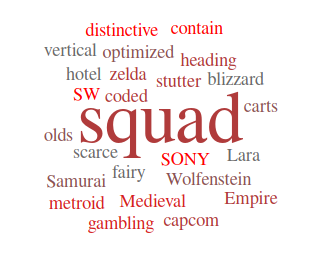
\includegraphics[width=\linewidth]{img/new_words2.png}
    \end{minipage}
    \titlecaption{ \centering  Word clouds}{Obtained by retrieving the attention scores of both modules.}
    \label{fig:att_adj_atr}
\end{figure}

\end{frame}
    \begin{frame}{Conclusion}
        \begin{itemize}
            \item Leveraging textual reviews $\rightarrow$ better performances
            \item Multi-task-learning $\rightarrow$ better performances
            \item The Attention mechanism $\rightarrow$ explainable predictions
        \end{itemize}
    \end{frame}
\end{section}